\chapter{Methodology}\label{ch:methodology}

This chapter describes the methodology to solve the problem. In \cref{sec:system_design}, the system design of the perception offloading is presented and explained. Then, the offloading strategies are described in \cref{sec:offloading_decision}. 

% -----------------------------------------------
\section{System Design}\label{sec:system_design}
% -----------------------------------------------

A perception offloading framework and different offloading strategies are designed and implemented in order to carry out the experiments. This section first describes the design for an offloading framework based on perception tasks. Then, different offloading strategies are presented. Finally, this section describes what system states are chosen to represent the state of the perception offloading.

\subsection{Perception offloading}

\begin{figure}[htp]
    \centering
    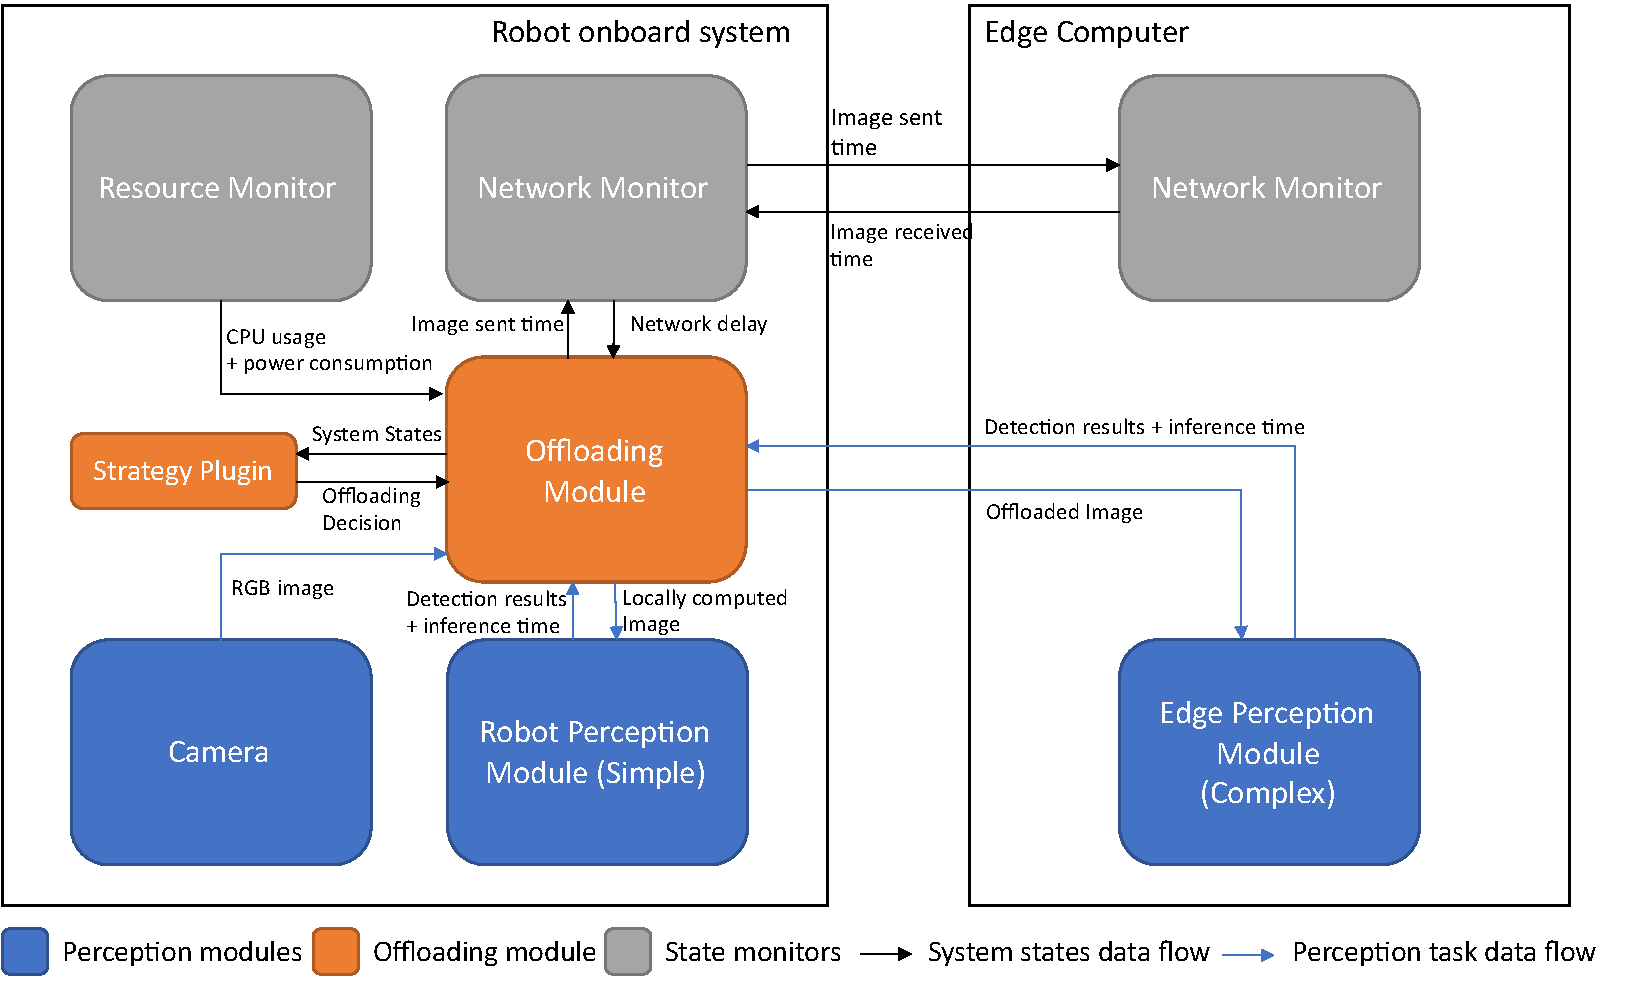
\includegraphics[width=\linewidth]{figures/setup/system_design.pdf}
    \caption[Design of perception offloading framework]{Design of perception offloading framework where the robot and the edge systems are separated by rectangles. Each system consists of different modules that are responsible for different tasks. The orange blocks represent modules related to offloading, while the blue blocks represent modules related to perception tasks. The grey blocks represent modules measuring system states. Arrows show the direction of data flows.}
    \label{fig:perception_offloading_framework}
\end{figure}

The designed offloading framework is illustrated in \cref{fig:perception_offloading_framework}. As shown, only the scenario where one \gls{amr} offloads the perception task to one edge computer is investigated. Therefore, the offloading modules are located solely on the robot's onboard system. To ensure the safety of the robot in case of a complete network connection loss, a perception module is also included on the robot's onboard system. However, since the robot onboard system usually has limited resources, the onboard perception module uses a less computationally expensive object detection model. In contrast, the edge computer has abundant resources. Therefore, it uses a perception module with a more complex model with higher precision. 

% Besides the processed detection, the perception modules also record the inference time used for each detection and return it to the offloading module. Furthermore, a network monitor is set up between the robot and the edge systems to measure the network latency. Finally, a resource monitor is used on the robot's onboard system to measure the onboard resource usage.

To evaluate different offloading strategies, the offloading module adopts a plug-in mechanism to load the offloading strategy at start-up. The offloading module receives different system states from the state monitors located on the robot's onboard system and on the edge computer. When the offloading module receives an image from the camera, it has to make a decision whether to offload the image to the edge computer or to compute it locally on the robot. Therefore, the offloading module passes the system states to the strategy plug-in as runtime parameters and receives the offloading decision. 

In addition to the perception modules and the offloading modules, there are also different state monitors that keep track of the onboard resources of the robot and the network condition between the robot and the edge computer. The network monitor measures the network latency between the robot and the edge computer. The resource monitor monitors CPU usage and energy consumption of the robot's onboard system. Furthermore, the perception modules are also responsible for measuring the inference times of the object detection models and sending them back to the offloading module 

\subsection{System States}

Various system states are considered for the perception offloading. They can be mainly divided into two categories: the onboard resources and the network condition. The network condition is measured by the network delay between the robot's onboard system and the edge computer. The outgoing data of the robot include the offloaded images with their sent times, while the incoming data contain an array of object detection results and the times when the edge computer receives the offloaded images and sends the detection back. The network monitors measure both the outgoing and incoming network delays. The total network delay can be calculated by

\begin{equation}
    t_{network} = t_{network}^{out} + t_{network}^{in}
\end{equation}

where $t_{network}^{out}$ is the network outgoing delay and the $t_{network}^{out}$ is the network outgoing delay. They can be calculated as

\begin{equation*}
    t_{network}^{out} = t_{sent}^{robot} - t_{received}^{edge}
\end{equation*}
\begin{equation*}
    t_{network}^{in} = t_{sent}^{edge} - t_{received}^{robot}
\end{equation*}

For onboard resource usage, the \gls{cpu} usage, the power consumption, and the bandwidth usage are measured. The \gls{cpu} usage and the power consumption can be directly measured with the robot's onboard system. However, the bandwidth usage needs to be calculated with the network IO measurements as follows:

\begin{equation}\label{eqn:bandwidth}
    bandwidth = \frac{n_{t_2} - n_{t_1}}{t_2 - t_1} \times 10^{-6} \times 8
\end{equation}

where $n_{t_i}$ represents the number of bytes the network has sent till time $t_i$. The bandwidth is calculated in megabits per second (Mbps). 

The onboard resource usage represents the availability of the \gls{amr}. If the \gls{cpu} usage is too high, the robot will have no resources left for other tasks performed onboard, such as \gls{slam} and navigation, and cannot operate anymore. Similarly, if the power consumption is too high, the robot needs to be recharged more often. Moreover, if the available bandwidth of the robot network is too small, the robot cannot communicate via the network. Therefore, these measurements are used as system states for making offloading decisions. 

% ----------------------------------------------------------
\section{Offloading Decision}\label{sec:offloading_decision}
% ----------------------------------------------------------

For the offloading module to make offloading decisions, an offloading strategy is needed. Several naive strategies are first investigated as baseline strategies. Their influence on various metrics of the system is evaluated. Based on their performance, a dynamic offloading strategy that uses the runtime system states, which are described in \cref{sec:system_design}, is implemented and evaluated against the baseline strategies. 

\subsection{Baseline strategies}

As baselines, the scenarios where the robot only computes the object detection task locally on its onboard system or only offloads the task to the edge computer are first investigated. These two strategies are named the "robot only" strategy and the "edge only" strategy. Then, the thesis continues to investigate the scenarios where the robot offloads a portion of the frames with a fixed ratio. For example, an offloading ratio of 0.2 will allows the offloading module to offload one image to the edge for every five images. The offloading strategies with a fixed offloading ratio can be realized with \cref{alg:ratio_strategy}. The offloading ratio should be a value ranging from 0 to 1. 

\begin{algorithm}[htp]
\caption{Algorithm to offload with a fixed ratio}\label{alg:ratio_strategy}
\begin{algorithmic}[1]
    \Function{RatioStrategy}{$r$} \Comment{where r is the offloading ratio}
        \State $c_1 \gets \, $GetImageCounter()\Comment{Get the counter for the total images received}
        \State $c_2 \gets \, $GetOffloadCounter()\Comment{Get the counter for the images offloaded}
        \State SetImageCounter($c_1 + 1$) \Comment{Add one first to image counter to avoid zero division}
        \If{$c_2 / c_1 \ge r$}
            \State return false \Comment{Compute locally}
        \Else
            \State SetOffloadCounter($c_2 + 1$)
            \State return true \Comment{Offload to edge computer}
        \EndIf
    \EndFunction
\end{algorithmic}
\end{algorithm}

With results from the experiments on baseline offloading strategies, this thesis intends to find the limits of the system and analyze its behavior. More specifically, the experiments and evaluation with the baseline strategies intend to investigate the question that under what circumstances the performance of the perception performance starts to deteriorate and offloading the perception tasks is no longer beneficial for the robot. With the results, a dynamic offloading strategy that uses runtime system states to make offloading decisions is then developed and implemented. 

\subsection{Dynamic offloading}

The dynamic offloading strategy aims to adapt to the changes in robot and edge systems as well as in network conditions. For the one-robot-one-edge scenario, a dynamic offloading strategy with the goal of minimizing the execution latency and improving the average precision of the object detection task is used. Moreover, this dynamic offloading strategy is subjected to the constraints of other system states. Two runtime system states are considered as constraints: \gls{amr}'s \gls{cpu} usage and the network bandwidth. The problem can be formulated as a constraint optimization problem as follow:

\begin{equation}\label{eqn:execution_latency}
    \min_{(\alpha, \beta)} \: t_{latency} = t_{inference} + t_{network}
\end{equation}

with

\begin{equation*}
    t_{inference} = \alpha t_{inference}^{L} + \beta t_{inference}^{E}
\end{equation*}
\begin{equation*}
    t_{network} = \alpha t_{network}^{L} + \beta t_{network}^{E}
\end{equation*}

s.t.

\begin{equation*}
    \alpha + \beta = 1
\end{equation*}

\begin{align*}
    & \alpha = \begin{cases}
        1, & \text{if the task is processed locally} \\
        0, & \text{else.}
    \end{cases} \\
    & \beta = \begin{cases}
        1, & \text{if the task is processed by the edge computer} \\
        0, & \text{else.}
    \end{cases}
\end{align*}

where the $t_{latency}$ represents the overall execution latency of the object detection task and $t_{inference}$ and $t_{network}$ represent the inference time and the network delay correspondingly. The execution latency is also called the \acrlong{rtt}. It measures the time for a round trip from the offloading module to the perception modules either located on the robot's onboard system or on the edge computer. 

In addition to the execution latency, the offloading decision is also subjected to the \gls{amr}'s \gls{cpu} usage and the network throughput. If the \gls{cpu} usage exceeds a certain value, the \gls{amr} only offloads to the edge. Similarly, the \gls{amr} only computes the task locally if the network throughput exceeds the threshold. These constraints ensure that the \gls{amr} and the network are capable of finishing the task at all. The decision-making strategy can be implemented as \cref{alg:decision_making_strategy}.

\begin{algorithm}[htp]
\caption{Algorithm to offload with dynamic parameters}\label{alg:decision_making_strategy}
\begin{algorithmic}[1]
    \Function{DecisionMakingStrategy}{$params$}\Comment{runtime parameters: $params$}
        \State $cpu_{max} \gets$ GetMaxCPULevel()
        \If{params['cpu\textunderscore usage'] $\geq cpu_{max}$} 
            \State return true \Comment{Offload if CPU usage exceeds limit}
        \EndIf
        \State $throughput_{max} \gets$ GetMaxThroughput()
        \If{params['bandwidth'] $\geq throughput_{max}$}
            \State return false \Comment{Compute locally if bandwidth usage exceeds limit}
        \EndIf
        
        \State $latency_{robot} \gets $ params['robot\textunderscore inference\textunderscore time'] + params['robot\textunderscore network\textunderscore delay']
        \State $latency_{edge} \gets $ params['edge\textunderscore inference\textunderscore time'] + params['edge\textunderscore network\textunderscore delay']
        \If{$latency_{robot} \geq latency_{edge}$}
            \State return true \Comment{Offload if edge RTT is higher}
        \Else
            \State return false \Comment{Compute locally if edge RTT is higher}
        \EndIf
    \EndFunction
\end{algorithmic}
\end{algorithm}
